\begin{figure}
\centering
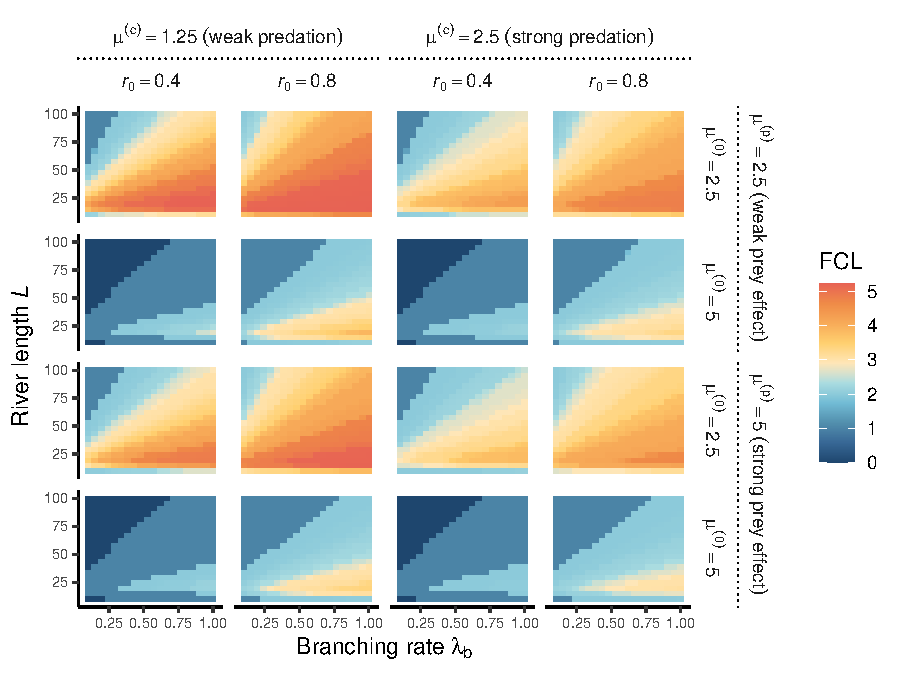
\includegraphics{../data_fmt/fig_rho025_g75_theta025.pdf}
\caption{Numerical prediction with low propagule \(g_0 = 75\), low
synchrony \(\rho = 0.25\), and weak omnivory \(\theta = 0.25\). Heatmaps
of FCL are expressed as a function of ecosystem size (river length,
\(L\)) and complexity (branching rate, \(\lambda_b\)), with rows and
columns displaying different combinations of resource supply (\(r_0\)),
disturbance regime (\(\mu^{(0)}\)), predation effect (\(\mu^{(c)}\)),
and prey effect (\(\mu^{(p)}\)). Each cell represents the average FCL of
five food webs. Additional parameter values are: habitat density
\(h=2.5\), dispersal capability \(\delta_0=0.5\), and scaling exponent
\(\psi_1=\psi_2=0.5\).\label{fig:fig-num1}}
\end{figure}

\newpage

\begin{figure}
\centering
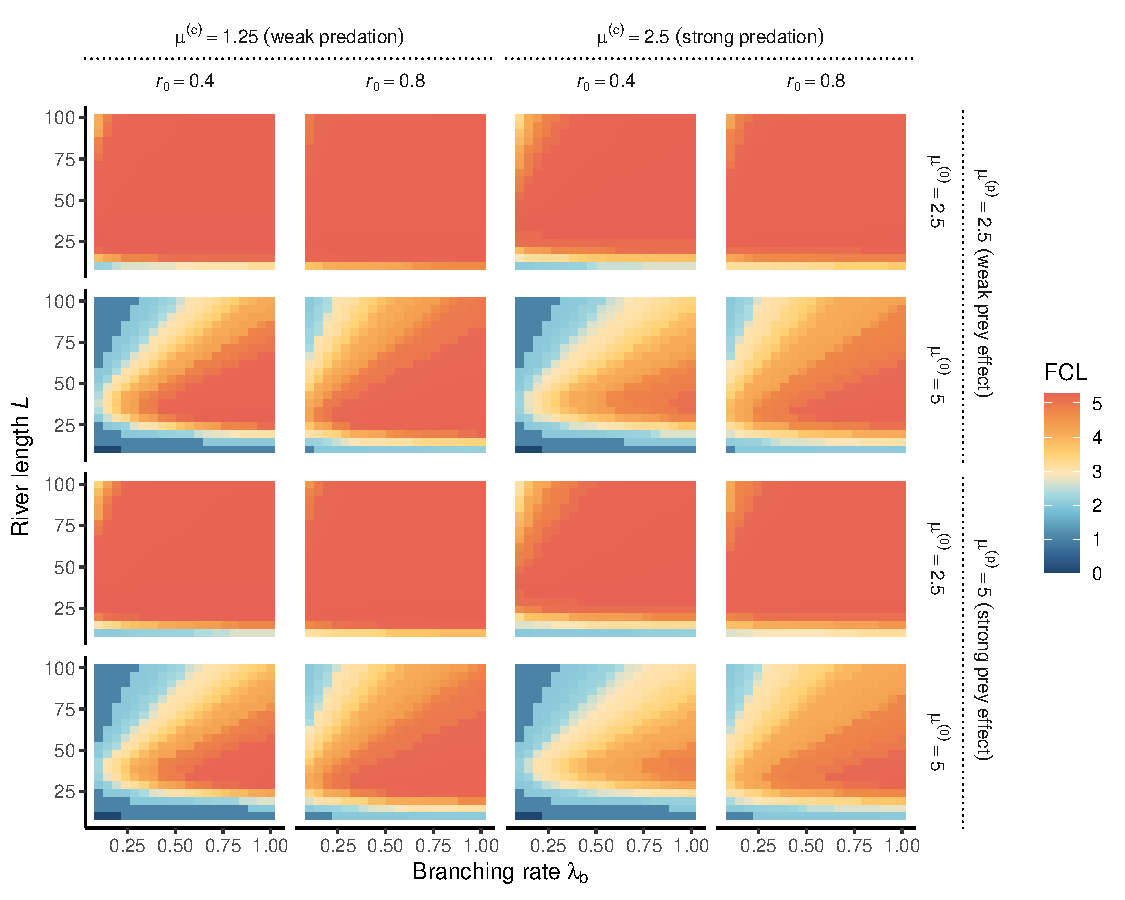
\includegraphics{../data_fmt/fig_rho025_g150_theta025.pdf}
\caption{Numerical prediction with high propagule \(g_0 = 150\), low
synchrony \(\rho = 0.25\), and weak omnivory \(\theta = 0.25\). Heatmaps
of FCL are expressed as a function of ecosystem size (river length,
\(L\)) and complexity (branching rate, \(\lambda_b\)), with rows and
columns displaying different combinations of resource supply (\(r_0\)),
disturbance regime (\(\mu^{(0)}\)), predation effect (\(\mu^{(c)}\)),
and prey effect (\(\mu^{(p)}\)). Each cell represents the average FCL of
five food webs. Additional parameter values are: habitat density
\(h=2.5\), dispersal capability \(\delta_0=0.5\), and scaling exponent
\(\psi_1=\psi_2=0.5\).\label{fig:fig-num2}}
\end{figure}

\newpage

\begin{figure}
\centering
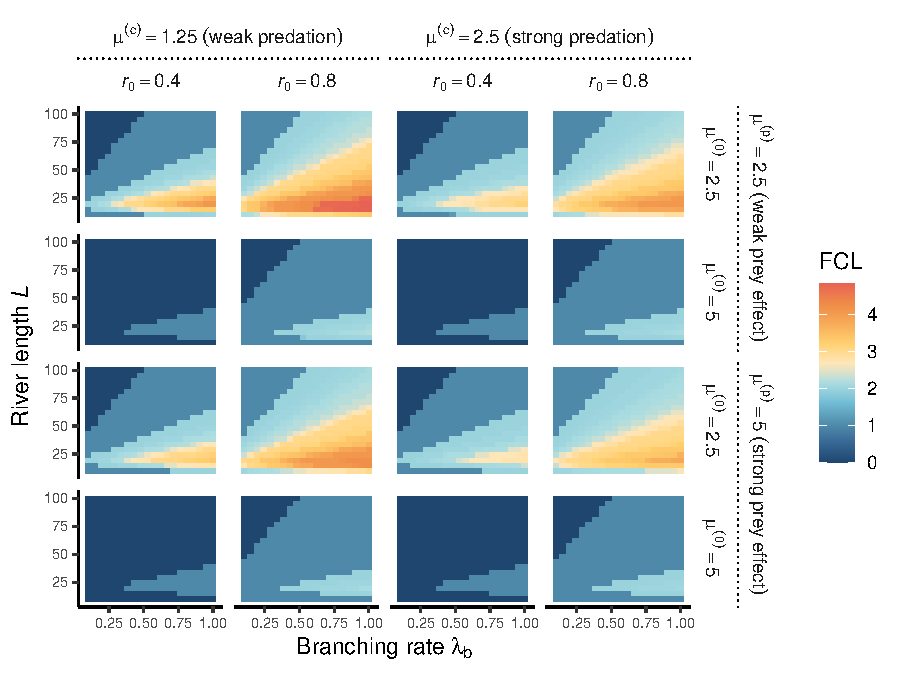
\includegraphics{../data_fmt/fig_rho05_g75_theta025.pdf}
\caption{Numerical prediction with low propagule \(g_0 = 75\), high
synchrony \(\rho = 0.5\), and weak omnivory \(\theta = 0.25\). Heatmaps
of FCL are expressed as a function of ecosystem size (river length,
\(L\)) and complexity (branching rate, \(\lambda_b\)), with rows and
columns displaying different combinations of resource supply (\(r_0\)),
disturbance regime (\(\mu^{(0)}\)), predation effect (\(\mu^{(c)}\)),
and prey effect (\(\mu^{(p)}\)). Each cell represents the average FCL of
five food webs. Additional parameter values are: habitat density
\(h=2.5\), dispersal capability \(\delta_0=0.5\), and scaling exponent
\(\psi_1=\psi_2=0.5\).\label{fig:fig-num3}}
\end{figure}

\newpage

\begin{figure}
\centering
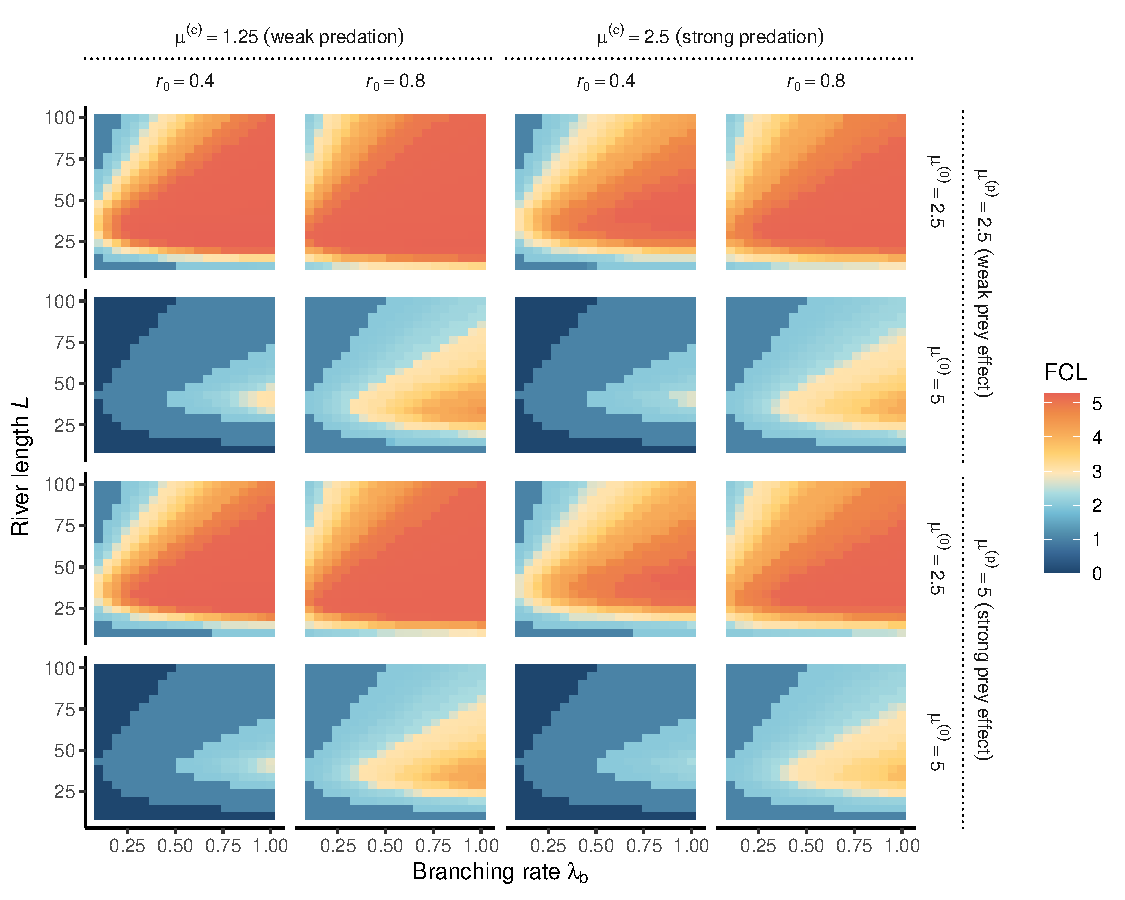
\includegraphics{../data_fmt/fig_rho05_g150_theta025.pdf}
\caption{Numerical prediction with high propagule \(g_0 = 150\), high
synchrony \(\rho = 0.5\), and weak omnivory \(\theta = 0.25\). Heatmaps
of FCL are expressed as a function of ecosystem size (river length,
\(L\)) and complexity (branching rate, \(\lambda_b\)), with rows and
columns displaying different combinations of resource supply (\(r_0\)),
disturbance regime (\(\mu^{(0)}\)), predation effect (\(\mu^{(c)}\)),
and prey effect (\(\mu^{(p)}\)). Each cell represents the average FCL of
five food webs. Additional parameter values are: habitat density
\(h=2.5\), dispersal capability \(\delta_0=0.5\), and scaling exponent
\(\psi_1=\psi_2=0.5\).\label{fig:fig-num4}}
\end{figure}

\newpage

\begin{figure}
\centering
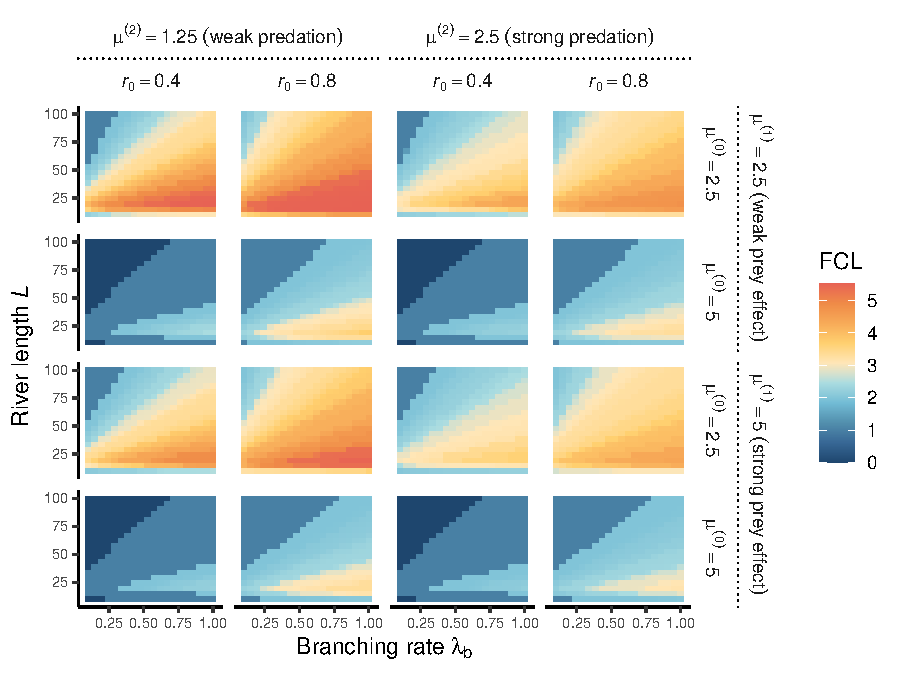
\includegraphics{../data_fmt/fig_rho025_g75_theta05.pdf}
\caption{Numerical prediction with low propagule \(g_0 = 75\), low
synchrony \(\rho = 0.25\), and strong omnivory \(\theta = 0.5\).Heatmaps
of FCL are expressed as a function of ecosystem size (river length,
\(L\)) and complexity (branching rate, \(\lambda_b\)), with rows and
columns displaying different combinations of resource supply (\(r_0\)),
disturbance regime (\(\mu^{(0)}\)), predation effect (\(\mu^{(c)}\)),
and prey effect (\(\mu^{(p)}\)). Each cell represents the average FCL of
five food webs. Additional parameter values are: habitat density
\(h=2.5\), dispersal capability \(\delta_0=0.5\), and scaling exponent
\(\psi_1=\psi_2=0.5\).\label{fig:fig-num5}}
\end{figure}

\newpage

\begin{figure}
\centering
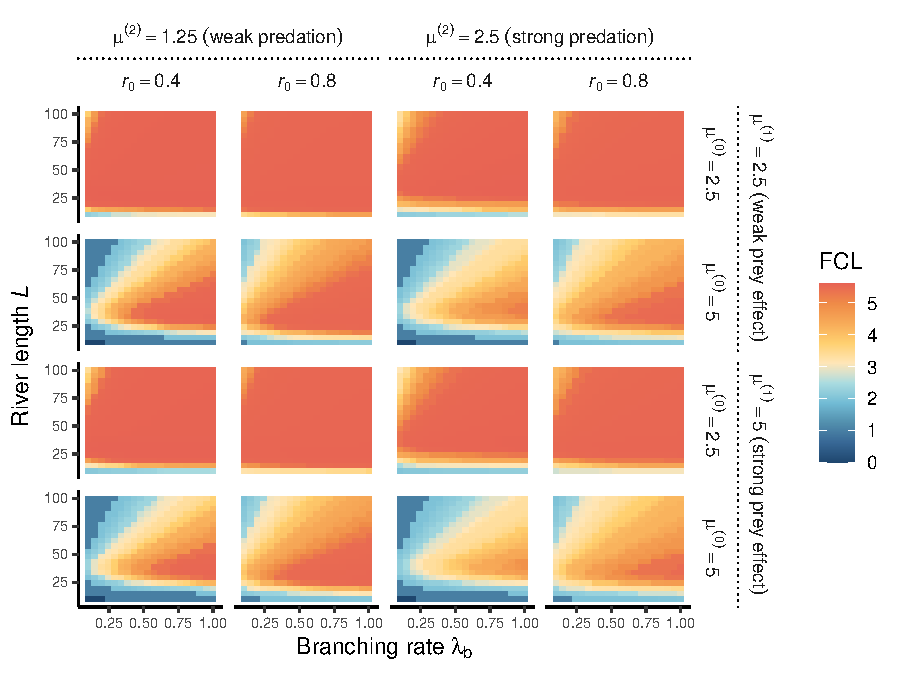
\includegraphics{../data_fmt/fig_rho025_g150_theta05.pdf}
\caption{Numerical prediction with high propagule \(g_0 = 150\), low
synchrony \(\rho = 0.25\), and strong omnivory \(\theta = 0.5\).Heatmaps
of FCL are expressed as a function of ecosystem size (river length,
\(L\)) and complexity (branching rate, \(\lambda_b\)), with rows and
columns displaying different combinations of resource supply (\(r_0\)),
disturbance regime (\(\mu^{(0)}\)), predation effect (\(\mu^{(c)}\)),
and prey effect (\(\mu^{(p)}\)). Each cell represents the average FCL of
five food webs. Additional parameter values are: habitat density
\(h=2.5\), dispersal capability \(\delta_0=0.5\), and scaling exponent
\(\psi_1=\psi_2=0.5\).\label{fig:fig-num6}}
\end{figure}

\newpage

\begin{figure}
\centering
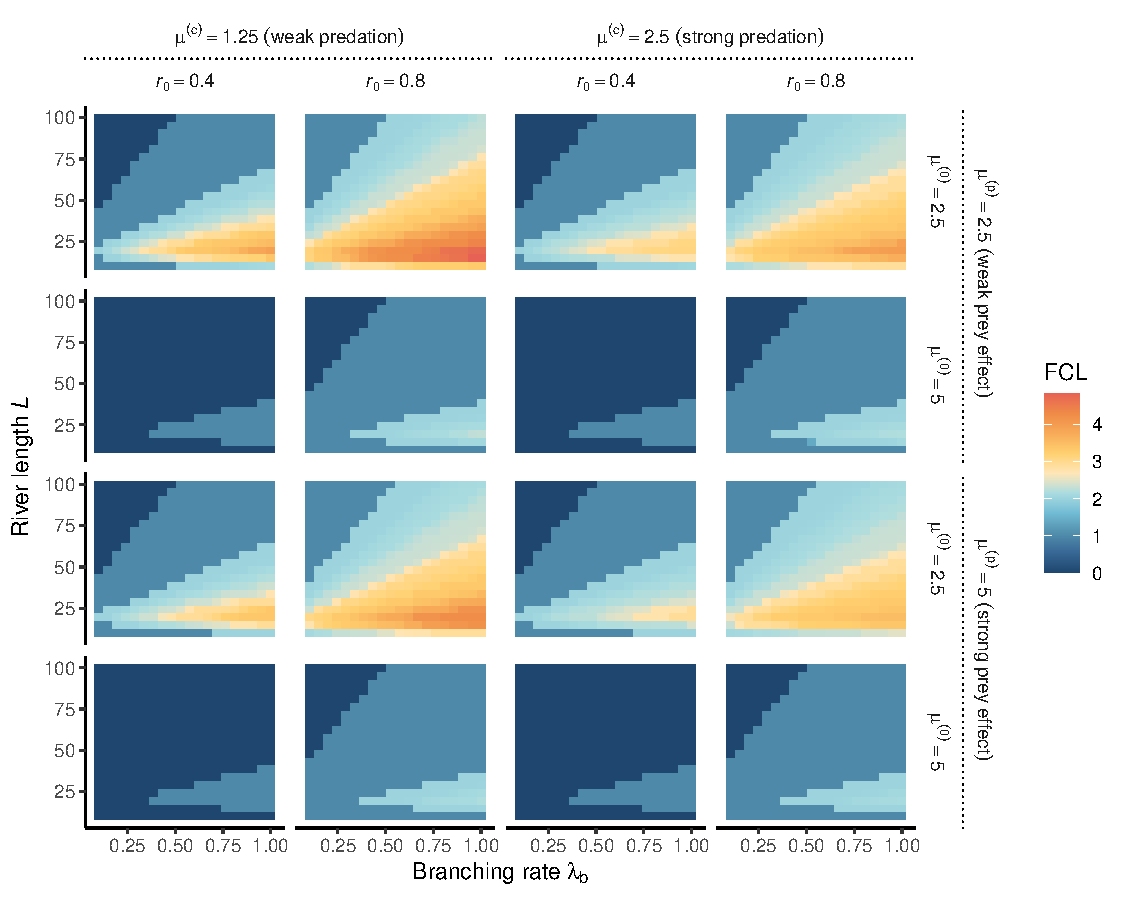
\includegraphics{../data_fmt/fig_rho05_g75_theta05.pdf}
\caption{Numerical prediction with low propagule \(g_0 = 75\), high
synchrony \(\rho = 0.5\), and strong omnivory \(\theta = 0.5\).Heatmaps
of FCL are expressed as a function of ecosystem size (river length,
\(L\)) and complexity (branching rate, \(\lambda_b\)), with rows and
columns displaying different combinations of resource supply (\(r_0\)),
disturbance regime (\(\mu^{(0)}\)), predation effect (\(\mu^{(c)}\)),
and prey effect (\(\mu^{(p)}\)). Each cell represents the average FCL of
five food webs. Additional parameter values are: habitat density
\(h=2.5\), dispersal capability \(\delta_0=0.5\), and scaling exponent
\(\psi_1=\psi_2=0.5\).\label{fig:fig-num7}}
\end{figure}

\newpage

\begin{figure}
\centering
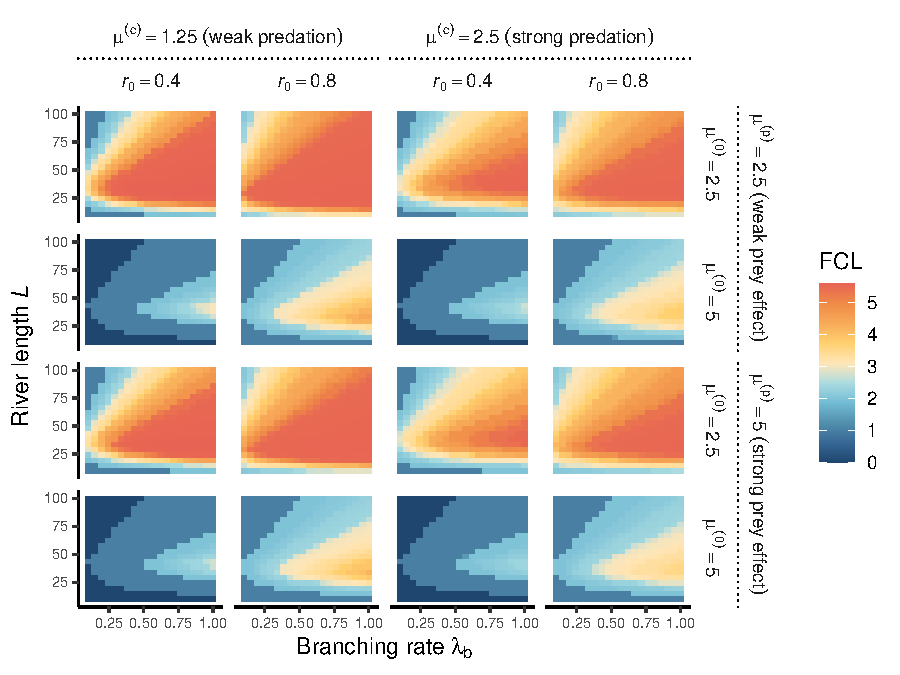
\includegraphics{../data_fmt/fig_rho05_g150_theta05.pdf}
\caption{Numerical prediction with high propagule \(g_0 = 150\), high
synchrony \(\rho = 0.5\), and strong omnivory \(\theta = 0.5\).Heatmaps
of FCL are expressed as a function of ecosystem size (river length,
\(L\)) and complexity (branching rate, \(\lambda_b\)), with rows and
columns displaying different combinations of resource supply (\(r_0\)),
disturbance regime (\(\mu^{(0)}\)), predation effect (\(\mu^{(c)}\)),
and prey effect (\(\mu^{(p)}\)). Each cell represents the average FCL of
five food webs. Additional parameter values are: habitat density
\(h=2.5\), dispersal capability \(\delta_0=0.5\), and scaling exponent
\(\psi_1=\psi_2=0.5\).\label{fig:fig-num8}}
\end{figure}

\newpage
